\documentclass{article}

% Language setting
% Replace `english' with e.g. `spanish' to change the document language
\usepackage[english]{babel}

% Set page size and margins
% Replace `letterpaper' with `a4paper' for UK/EU standard size
\usepackage[letterpaper,top=2cm,bottom=2cm,left=3cm,right=3cm,marginparwidth=1.75cm]{geometry}

% Useful packages
\usepackage{amsmath}
\usepackage{graphicx}
\usepackage[colorlinks=true, allcolors=blue]{hyperref}

\title{Rapport}
\author{Jean-emmanuel Chouinard (20246807), Timothe Payette (20239892)}
\date{10 juillet 2023}

\begin{document}
\maketitle

\section{Auto-évaluation}

Notre programme fonctionne comme prévu. Il respecte les consignes et le format des sorties demandé. Le seul exemple où notre programme ne concorde pas à 100\% est l'exemple 6. Nous jugeons cela normal puisque le stock donné et la date courante permet d'utiliser ces médicaments. Voici des images de ces différences

\begin{figure}[htp]
\centering
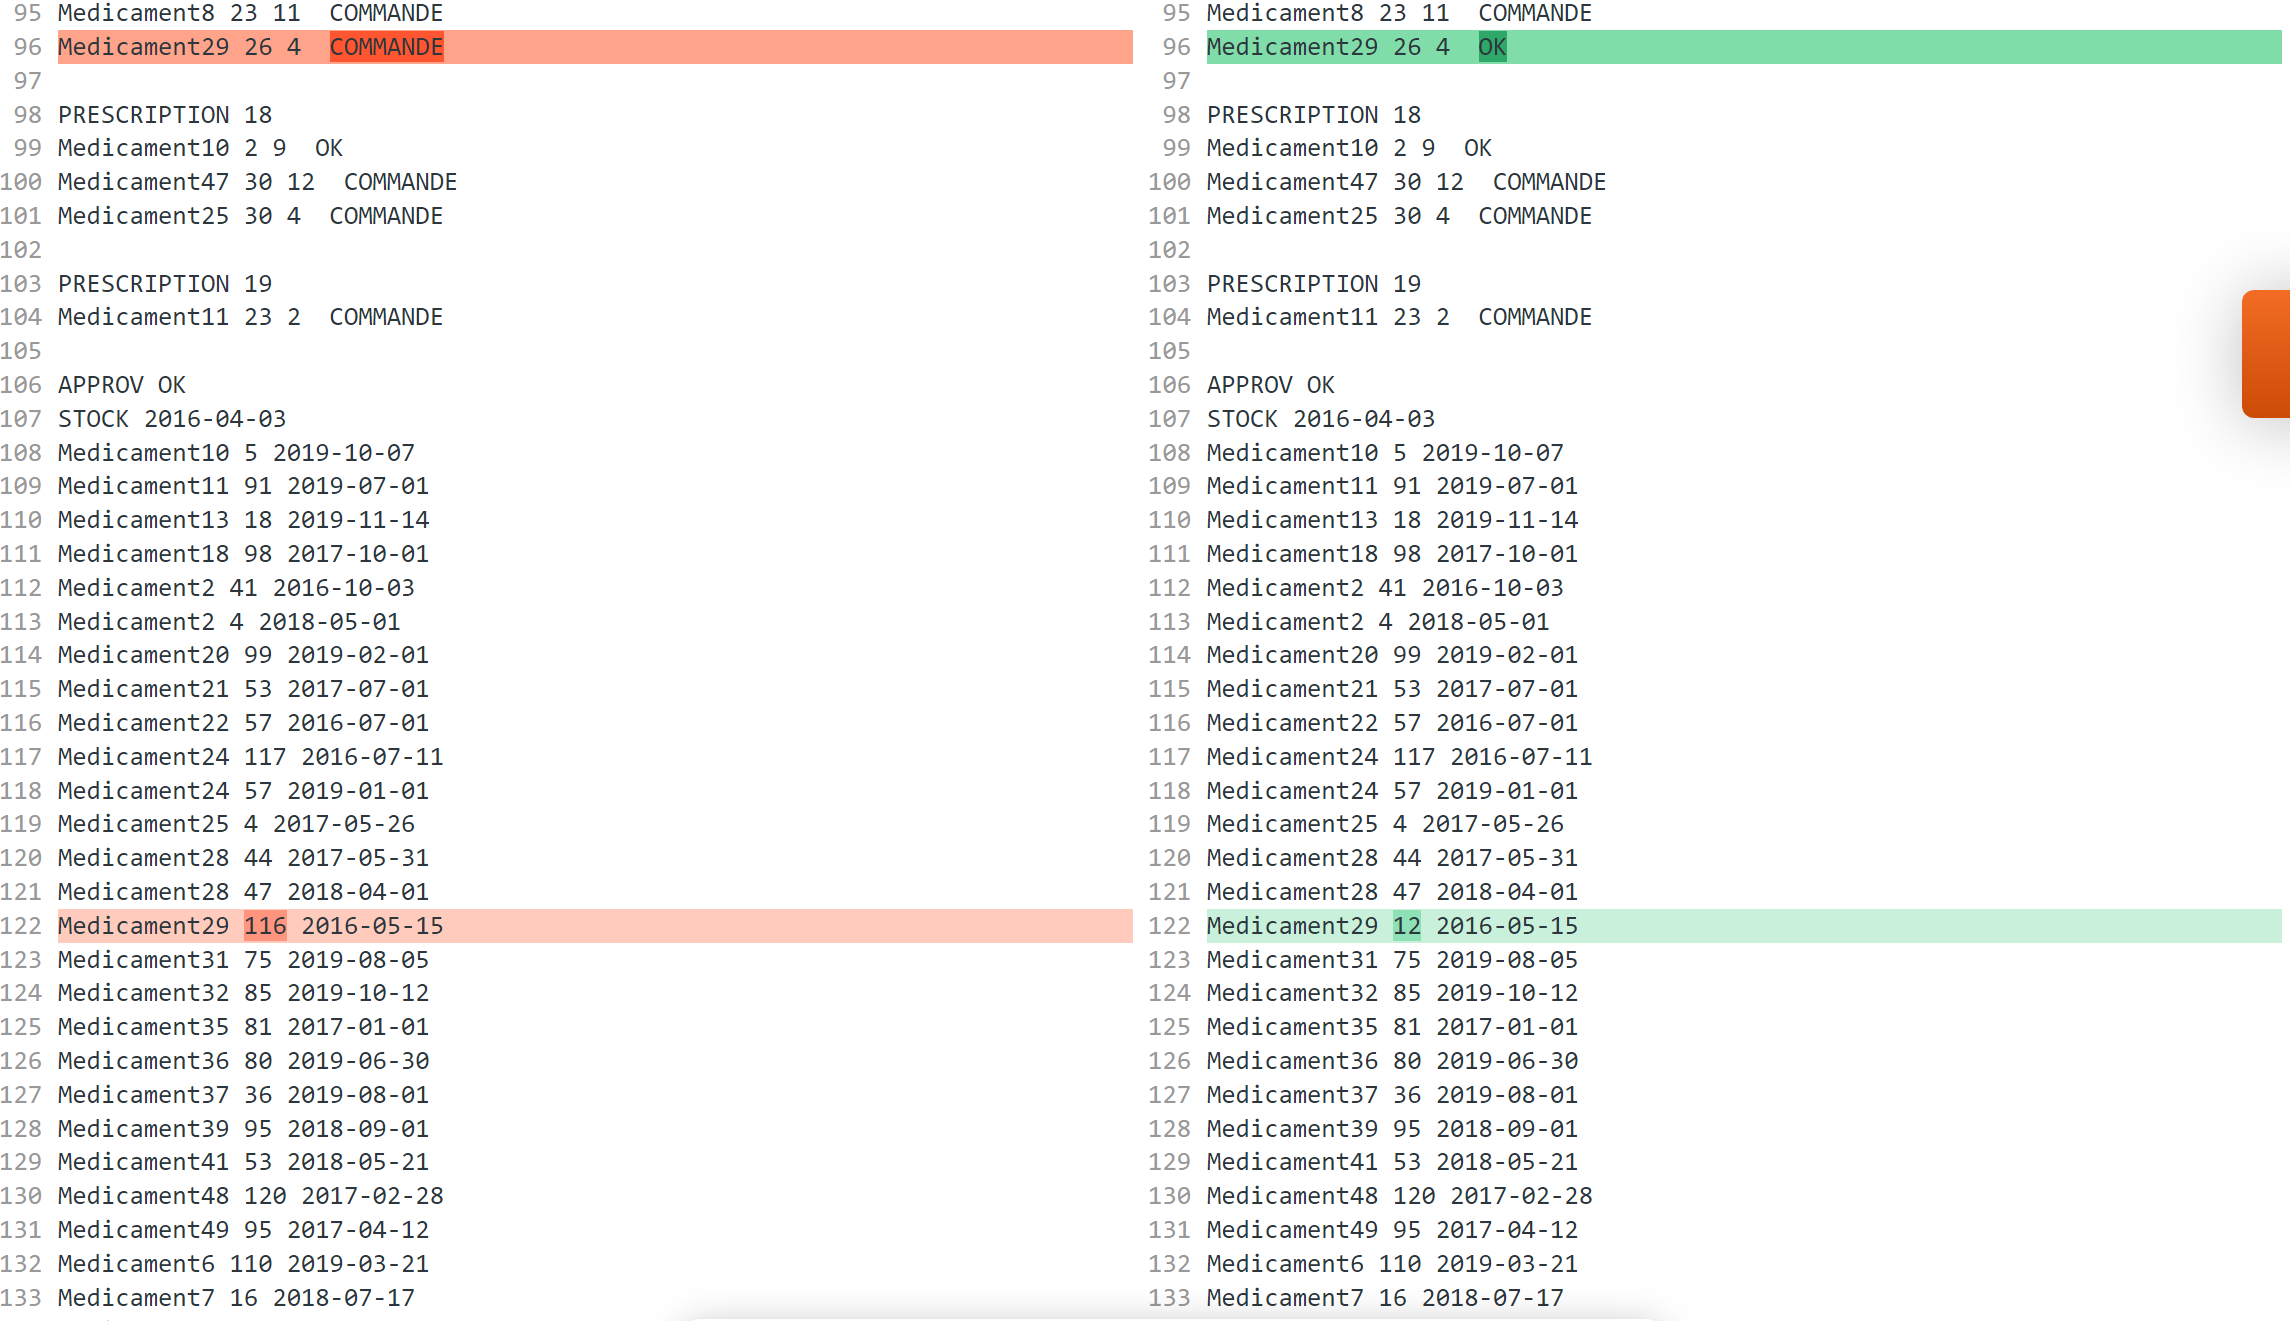
\includegraphics[width=0.5\textwidth]{Diff1.png}
\end{figure}

\begin{figure}[htp]
\centering
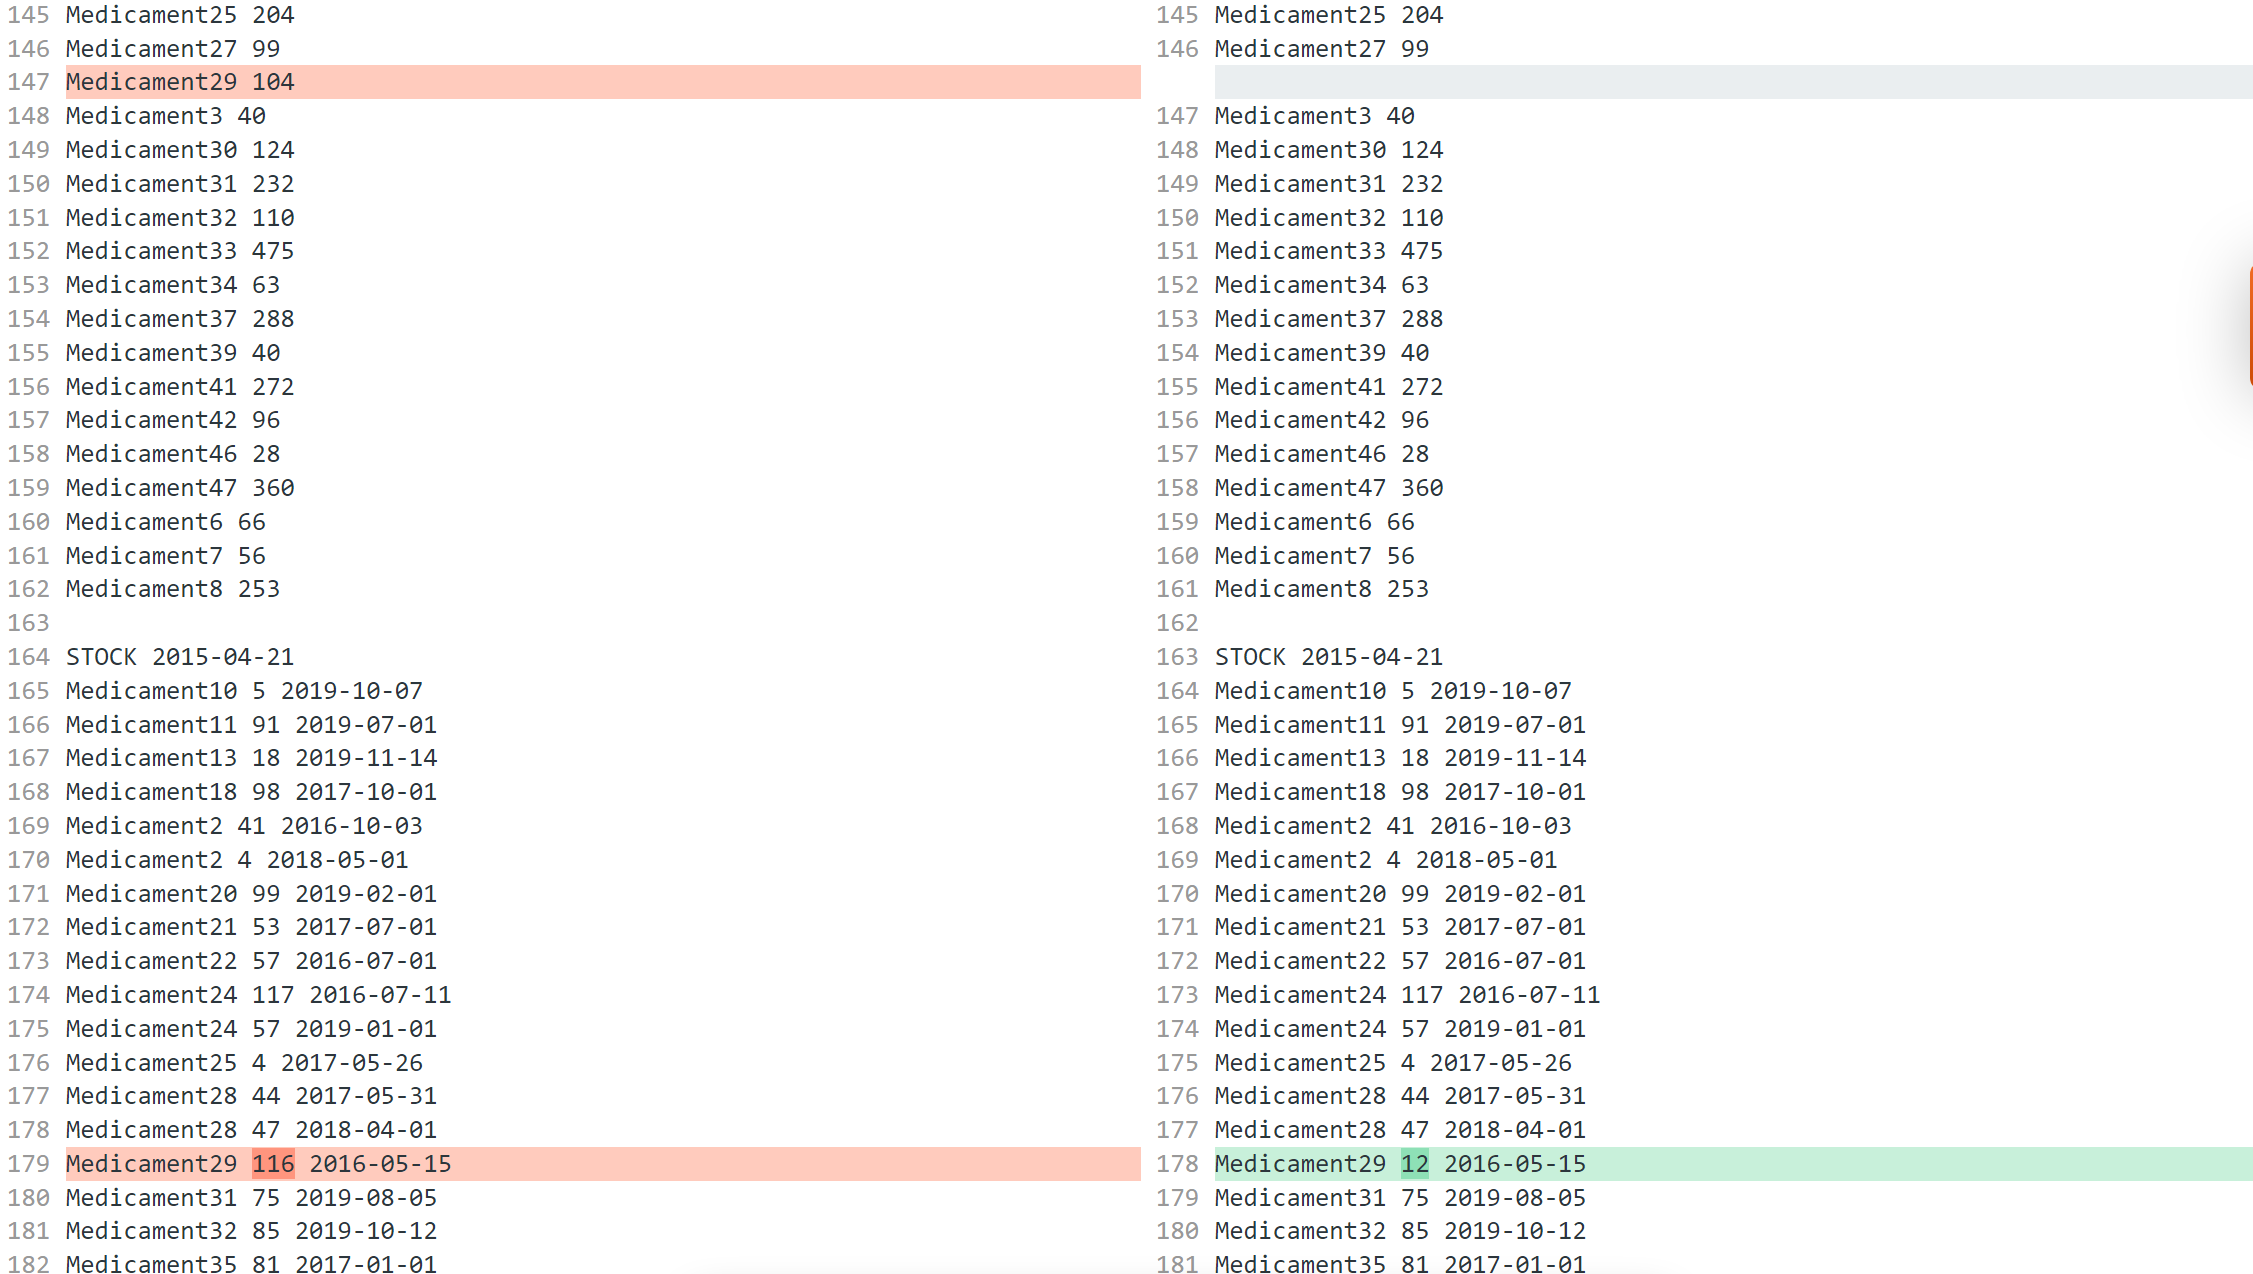
\includegraphics[width=0.5\textwidth]{Diff2.png}
\end{figure}

\section{Analyse de la complexité temporelle (pire cas) théorique en notation grand O}


\subsection{Légende}
Voici la légende que nous allons utiliser tout au long de l'analyse:
\begin{itemize}
    \item n - indique le nombre de types de médicaments différents en stock
    \item m - indique le nombre d'items sur la prescription
    \item k - indique le nombre d'items sur la liste de commande
    \item l - indique le nombre de médicaments à ajouter au stock
\end{itemize}


\subsection{Prescription}

Voici notre algorithme pour la fonction "Prescription"

\begin{figure}[htp]
\centering
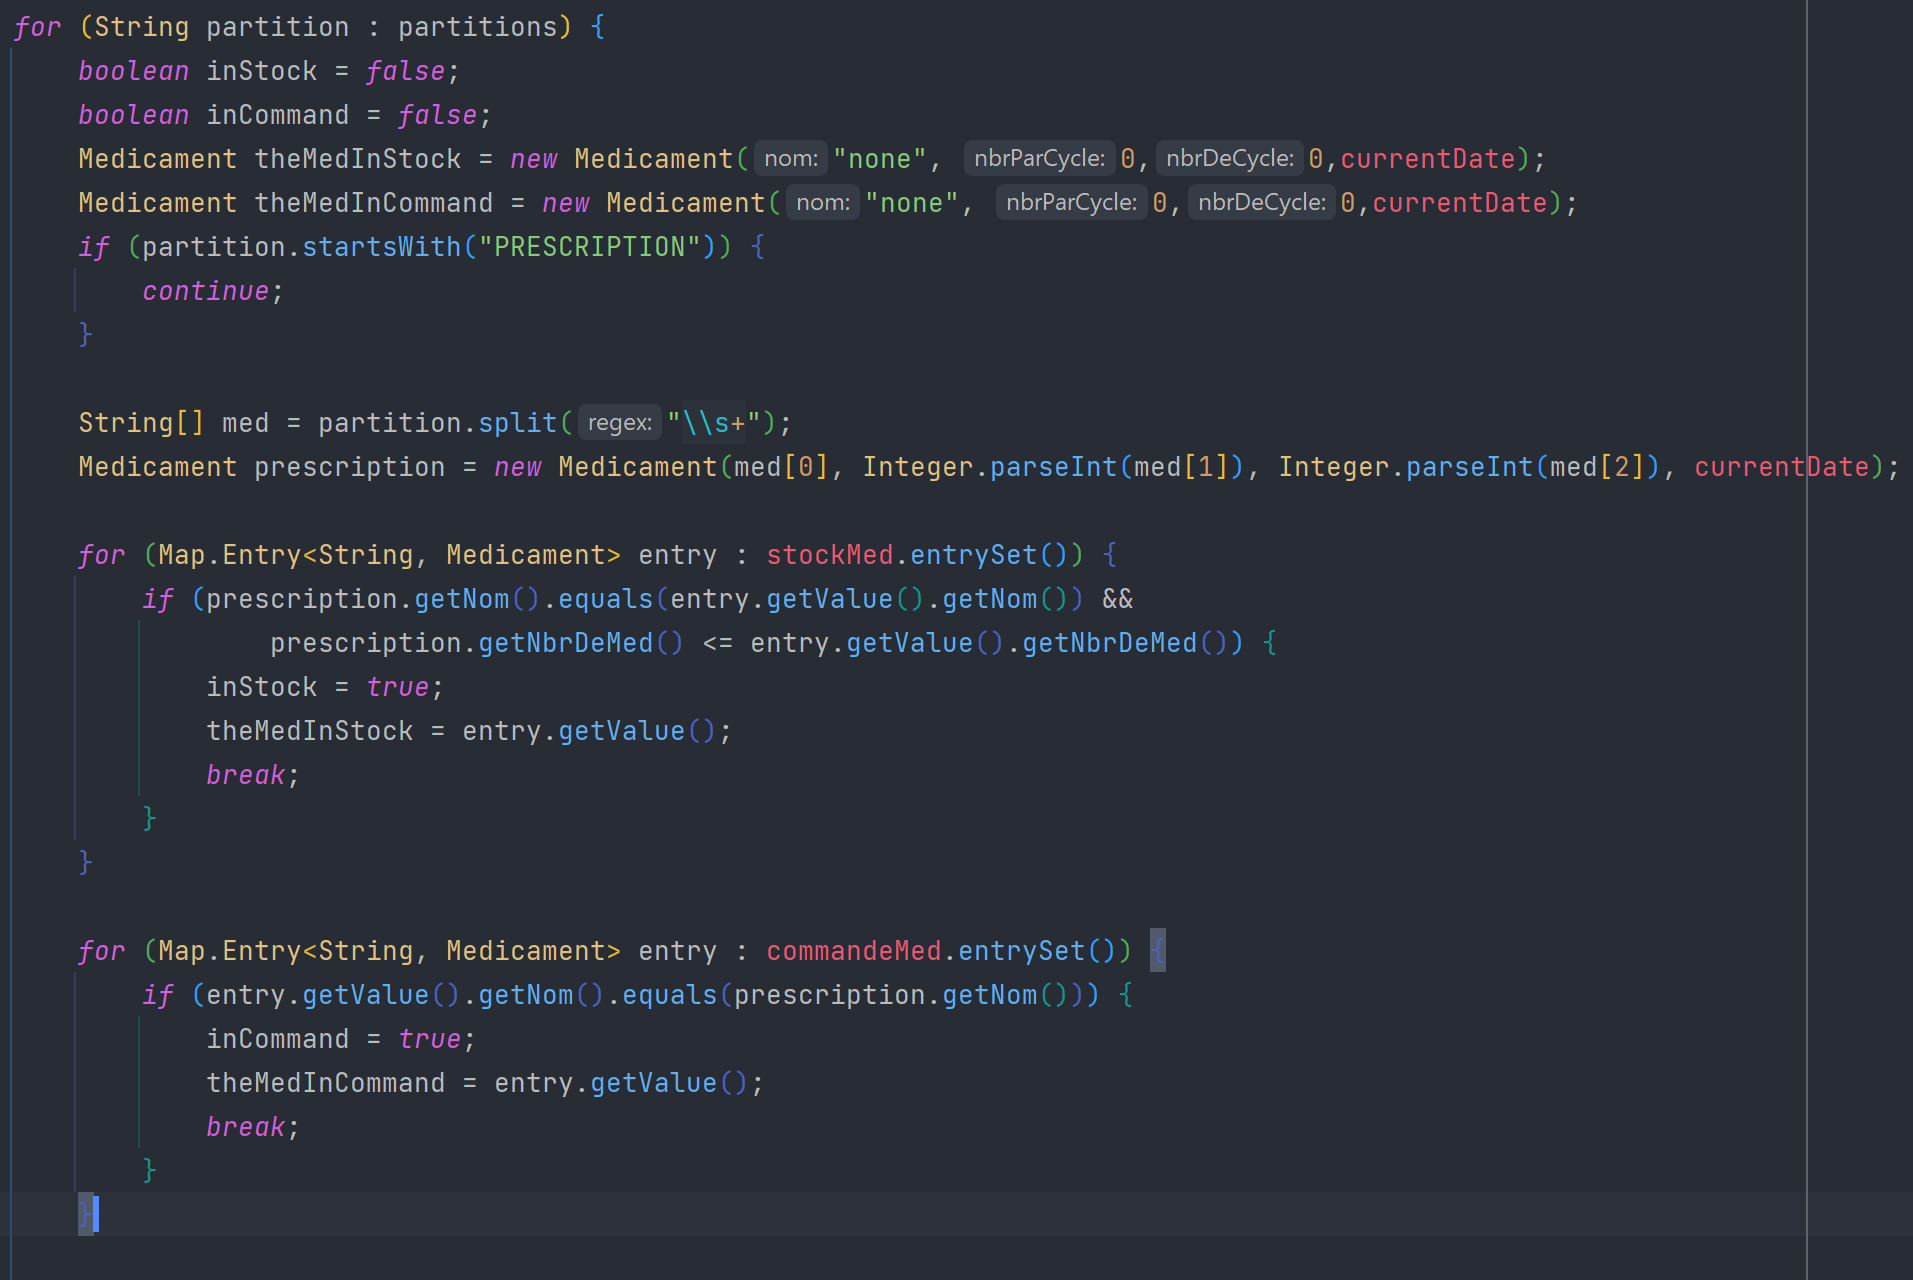
\includegraphics[width=0.5\textwidth]{Presc1.png}
\end{figure}

\begin{figure}[htp]
\centering
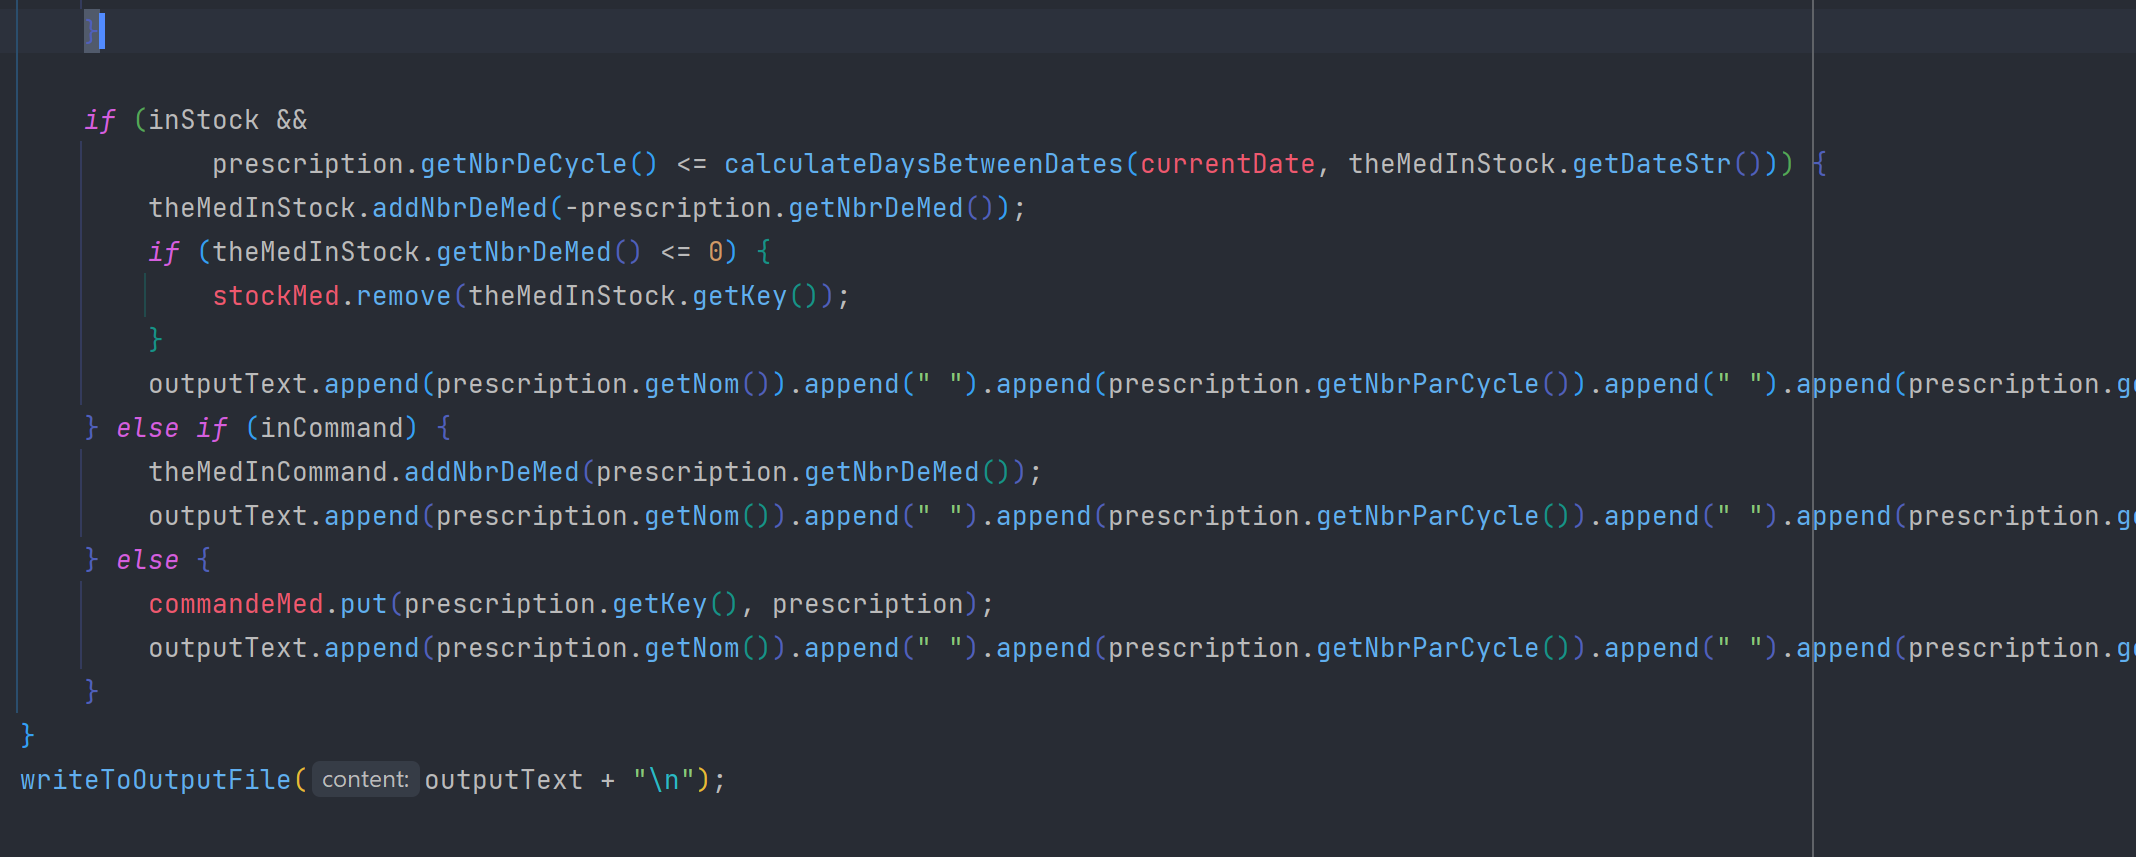
\includegraphics[width=0.5\textwidth]{Presc2.png}
\end{figure}

On voit que pour chaque item de la prescription ( O(m) ), deux boucles sont faites: une sur les médicaments en stock ( O(n) ) et une sur les médicaments déjà dans la commande ( O(k) ). Notre fonction se réalise donc en $O(m * (n+k))$.

\subsection{Approv}

Voici notre algorithme pour la fonction "Approv"

\begin{figure}[htp]
\centering
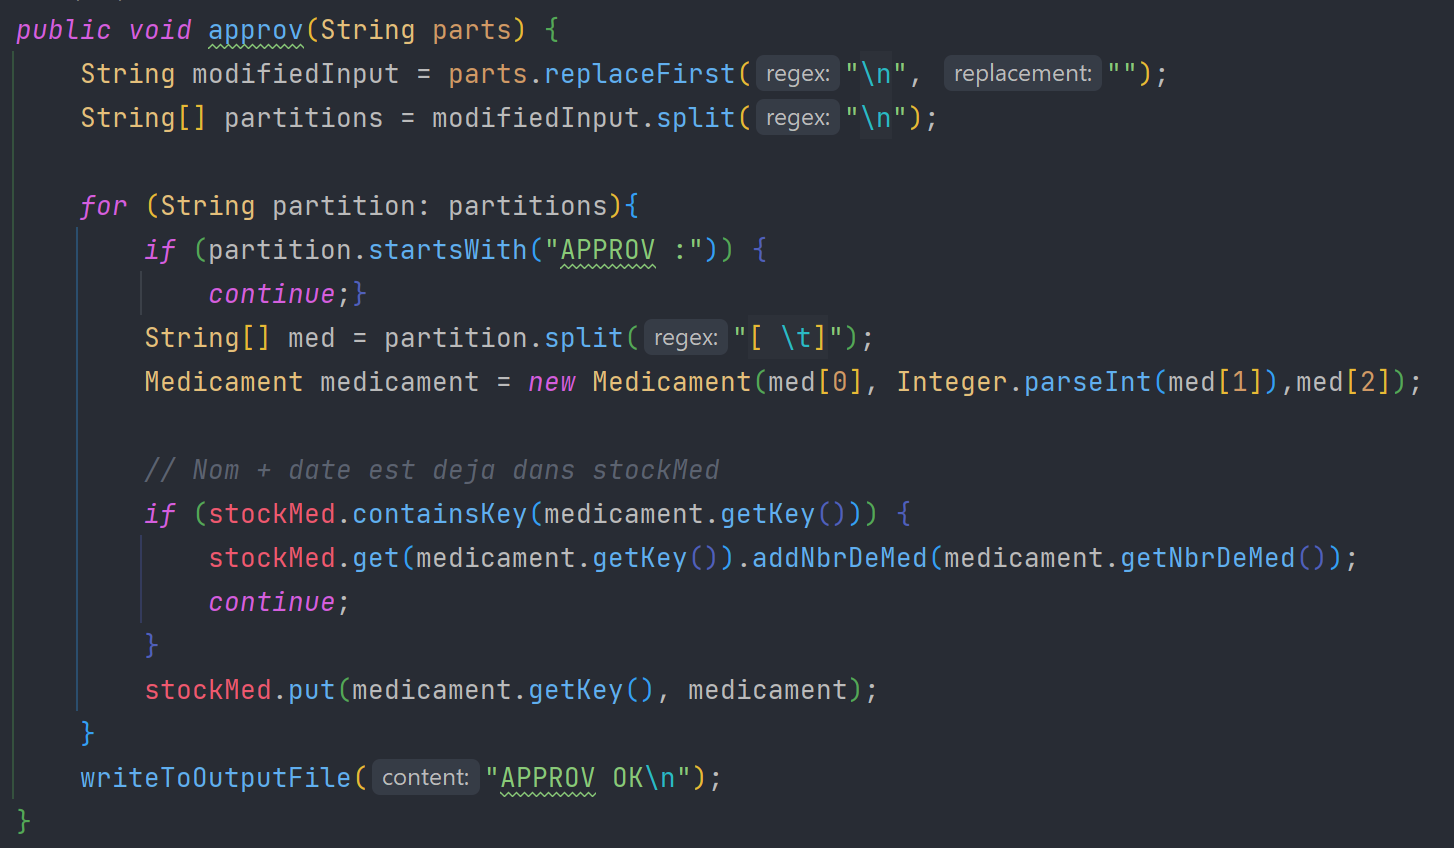
\includegraphics[width=0.5\textwidth]{Approv.png}
\end{figure}

On voit qu'une boucle passe à travers la liste d'ajout ( O(l) ). De plus, la fonction "contains" de l'arbre est utilisé pour trouver des éléments dans la liste de médicaments en stock ( O(logn) ). Notre fonction se réalise donc en $O(l*log(n))$. \\\\\\\\\\\\

\subsection{Date}

Voici notre algorithme pour la fonction "Date"

\begin{figure}[htp]
\centering
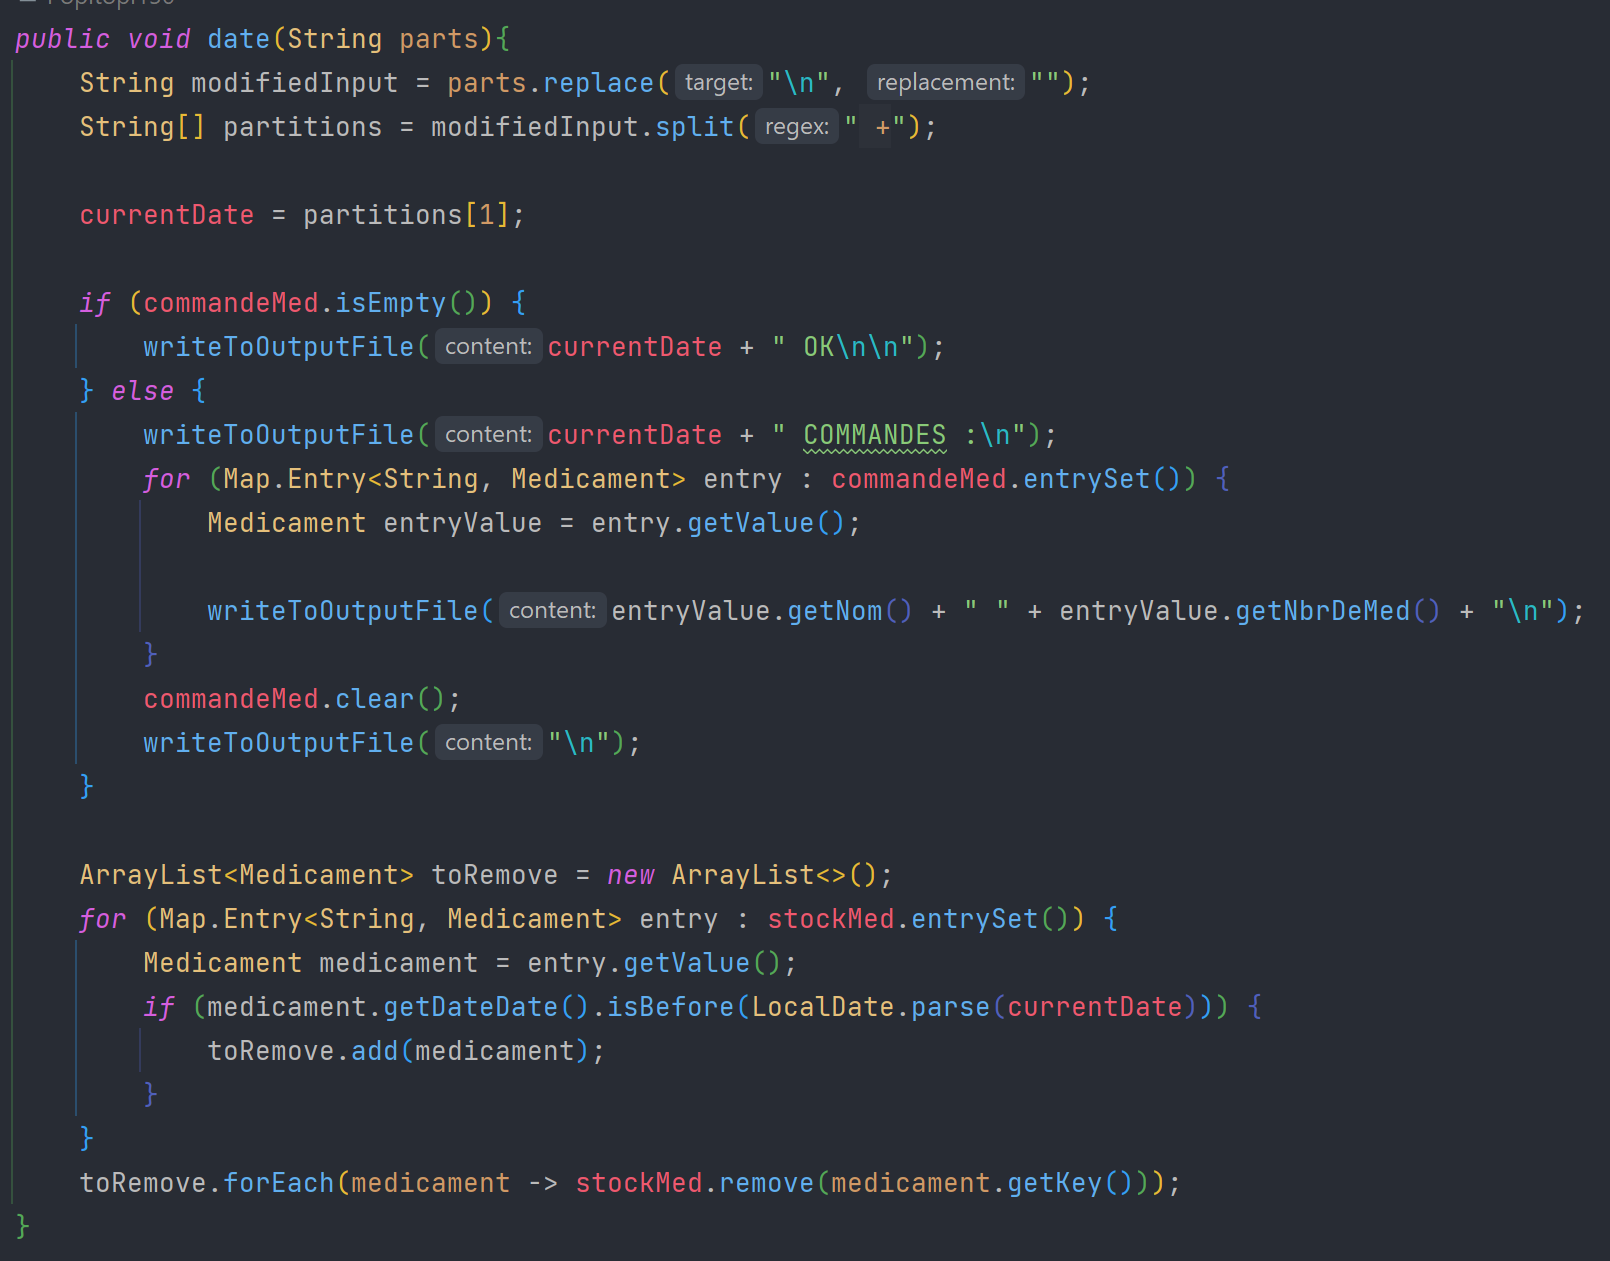
\includegraphics[width=0.5\textwidth]{Date.png}
\end{figure}

On voit qu'une boucle permet d'imprimer toutes les médicaments en commande ( O(k) ). Ensuite, on vérifie si des médicaments ont expirés et on les suppriment de l'arbre ( $O(n^2)$ ). Notre fonction se réalise donc en $O(k*n^2)$. 

\end{document}